\documentclass[border=6pt]{standalone}
\usepackage{amsmath,amssymb}
\usepackage{tikz}
\usetikzlibrary{arrows.meta,shadows,calc,backgrounds}
\begin{document}
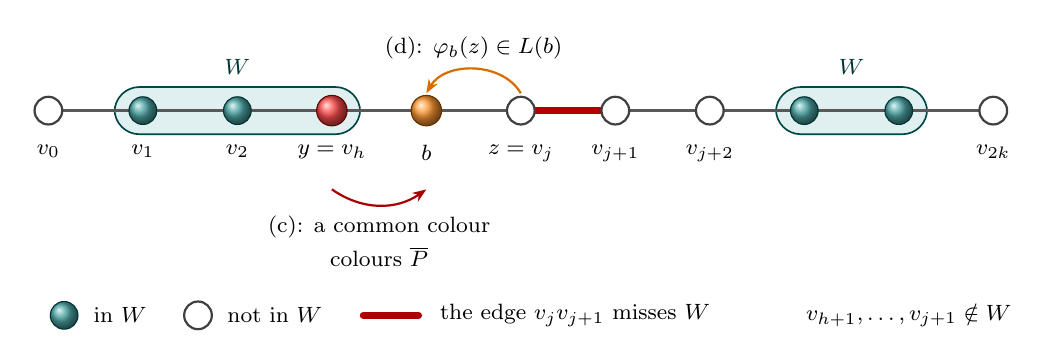
\begin{tikzpicture}[
  inW/.style={circle,inner sep=0pt,minimum size=10pt,ball color=teal!70,draw=teal!40!black,line width=0.4pt},
  outW/.style={circle,inner sep=0pt,minimum size=10pt,draw=black!75,line width=0.8pt,fill=white},
  yv/.style={circle,inner sep=0pt,minimum size=11pt,ball color=red!70,draw=red!40!black,line width=0.4pt},
  bv/.style={circle,inner sep=0pt,minimum size=11pt,ball color=orange!80,draw=orange!40!black,line width=0.4pt},
  pe/.style={line width=1.1pt,black!65},
  miss/.style={line width=2.6pt,red!70!black,line cap=round},
  blob/.style={rounded corners=9pt,fill=teal!12,draw=teal!55!black,line width=0.6pt},
  lab/.style={font=\footnotesize},
  note/.style={font=\footnotesize,align=center}]
\foreach \i in {0,...,10} { \coordinate (v\i) at (1.2*\i,0); }
% the minimal tight set W
\begin{scope}[on background layer]
  \draw[blob] ($(v1)+(-0.36,-0.3)$) rectangle ($(v3)+(0.36,0.3)$);
  \draw[blob] ($(v8)+(-0.36,-0.3)$) rectangle ($(v9)+(0.36,0.3)$);
\end{scope}
\draw[pe] (v0) -- (v10);
\draw[miss] (v5) -- (v6);
\foreach \i in {0,7,10} { \node[outW] at (v\i) {}; }
\foreach \i in {1,2,8,9} { \node[inW] at (v\i) {}; }
\node[yv] (y) at (v3) {};
\node[bv] (b) at (v4) {};
\node[outW] (z) at (v5) {};
\node[outW] at (v6) {};
% indices below
\foreach \i/\t in {0/v_0,1/v_1,2/v_2,7/v_{j+2},10/v_{2k}} { \node[lab,below=9pt] at (v\i) {$\t$}; }
\node[lab,below=9pt] at (v3) {$y=v_h$};
\node[lab,below=9pt] at (v4) {$b$};
\node[lab,below=9pt] at (v5) {$z=v_j$};
\node[lab,below=9pt] at (v6) {$v_{j+1}$};
\node[lab,teal!40!black] at ($(v2)+(0,0.55)$) {$W$};
\node[lab,teal!40!black] at ($($(v8)!0.5!(v9)$)+(0,0.55)$) {$W$};
% (c): shared colour between y and b
\draw[-{Stealth[length=5pt]},line width=0.8pt,red!65!black] ($(y)+(0,-1.0)$) to[bend right=35]
  node[below,note,black]{(c): a common colour\\[3pt] colours $\overline P$} ($(b)+(0,-1.0)$);
% (d): phi_b(z) lies in L(b)
\draw[-{Stealth[length=5pt]},line width=0.8pt,orange!85!black] ($(z)+(0,0.22)$) to[bend right=60]
  node[above,note,black]{(d): $\varphi_b(z)\in L(b)$} ($(b)+(0,0.22)$);
% legend
\node[inW] at (0.2,-2.6) {}; \node[lab,anchor=west] at (0.45,-2.6) {in $W$};
\node[outW] at (1.9,-2.6) {}; \node[lab,anchor=west] at (2.15,-2.6) {not in $W$};
\draw[miss] (4.0,-2.6) -- (4.7,-2.6); \node[lab,anchor=west] at (4.85,-2.6) {the edge $v_jv_{j+1}$ misses $W$};
\node[lab,anchor=west] at (9.5,-2.6) {$v_{h+1},\dots,v_{j+1}\notin W$};
\end{tikzpicture}
\end{document}
